% --------------------------------------------------------------
% This is all preamble stuff that you don't have to worry about.
% Head down to where it says "Start here"
% --------------------------------------------------------------

\documentclass[12pt]{article}

\usepackage[margin=1in]{geometry}
\usepackage{amsmath,amsthm,amssymb}
\usepackage{enumerate}
\usepackage{graphicx}
\usepackage[english]{babel}
\usepackage[utf8x]{inputenc}
\usepackage[T1]{fontenc}
\usepackage{enumitem}
\usepackage{fancyhdr}
\pagestyle{fancy}


\newcommand{\N}{\mathbb{N}}
\newcommand{\Z}{\mathbb{Z}}
\newcommand{\R}{\mathbb{R}}
\newcommand{\Q}{\mathbb{Q}}

\newenvironment{theorem}[2][Theorem]{\begin{trivlist}
\item[\hskip \labelsep {\bfseries #1}\hskip \labelsep {\bfseries #2.}]}{\end{trivlist}}
\newenvironment{lemma}[2][Lemma]{\begin{trivlist}
\item[\hskip \labelsep {\bfseries #1}\hskip \labelsep {\bfseries #2.}]}{\end{trivlist}}
\newenvironment{exercise}[2][Exercise]{\begin{trivlist}
\item[\hskip \labelsep {\bfseries #1}\hskip \labelsep {\bfseries #2.}]}{\end{trivlist}}
\newenvironment{problem}[2][Problem]{\begin{trivlist}
\item[\hskip \labelsep {\bfseries #1}\hskip \labelsep {\bfseries #2.}]}{\end{trivlist}}
\newenvironment{question}[2][Question]{\begin{trivlist}
\item[\hskip \labelsep {\bfseries #1}\hskip \labelsep {\bfseries #2.}]}{\end{trivlist}}
\newenvironment{corollary}[2][Corollary]{\begin{trivlist}
\item[\hskip \labelsep {\bfseries #1}\hskip \labelsep {\bfseries #2.}]}{\end{trivlist}}

\lhead{Homework 4, April 30, 2021}
\rhead{Nicholas Tee}

\begin{document}
Worked with: Brooke Zhang, Emily Louie
\subsection*{Problem 1}
In order to show that ~ is an equivalence relation on the group $G$ then we need to show that it is reflexive, symmetric and transitive:\\
\textit{Reflexive: } let $h \in G$, there will be an element $g \in G$ such that $h = ghg^{-1}$ which will end up as $h = h$. We can then say that $h \sim h$\\
\textit{Symmetric: } let $h,h' \in G$. We can say that there will be some element $g \in G$ such that $h  = gh'g^{-1}$. Then the reverse is also true which is $h' = ghg^{-1}$. We can then say that $h' \sim h$.\\
\textit{Transitive: } let $h,h'h'' \in G$. There there will be some elements $g,k \in G$ such that $h = gh'g^{-1}$ and $h'' = kh'k^{-1}$. This means that since $h = gh'g^{-1}$ we can say that $h'' = k(ghg^{-1})k^{-1} = (gk)h(gk)^{-1}$. Since $G$ is a group then $gk \in G$. Thus, $h \sim h''$
\subsection*{Problem 2}
\begin{proof}
Suppose $B_n$ is the set of all odd permutations in $S_n$. Let $\varphi: A_n \rightarrow B_n$, for some permutation $a \in A_n$, we can say that
\[
	\varphi(a) = (1 2)a
\]
Since we know that $a$ is an even permutation, $(1 2)a$ is odd, so $(1 2)a \in B_n$.\\
Now, let there be two permutations $a_1,a_2 \in A_n$. We can then show that $\varphi$ is injective as such
\[ \varphi(a_1) = \varphi(a_2) \]
\[ (12)\varphi(a_1) = (1 2)\varphi(a_2) \]
\[ (12)(12)\varphi(a_1) = (12)(12)\varphi(a_2) \]
Since $(1 2)(1 2) = e$, we get
\[ a_1 = a_2 \]
Thus $\varphi$ is injective. In order to show that is is surjective, let there be a permutation $b \in B_n$ such that $(1 2)b \in A_n$
\[ \varphi((1 2)b) \]
\begin{align*}
\varphi((12)b) &= (12)\cdot (12)b\\
 &= e \cdot b\\
 &= b
\end{align*}
With this we now know that $\varphi$ is surjective, meaning that there is a bijection between the sets $A_n$ and $B_n$. We can then say that $|A_n| = |B_n|$. Since, $A_n \cup B_n = S_n$, and that $|S_n| = n!$, we can then say that $|A_n| = \frac{n!}{2}$ as it would be exactly half the size of $S_n$.
\end{proof}
\newpage
\subsection*{Problem 3}
Since we have 3 different elements of order 2 in each group, if we try to pair the elements together, there would be 6 different isomorphisms between $K_4$ and $\Z/2\Z \times \Z/2\Z$. (For all 6 isomorphisms (0,0) will map to the identity element)\\
\textbf{First:}
\begin{align*}
(0,1) &\rightarrow (12)(34)\\
(1,0) &\rightarrow (13)(24)\\
(1,1) &\rightarrow (14)(23)
\end{align*}
\textbf{Second:}
\begin{align*}
(0,1) &\rightarrow (12)(34)\\
(1,0) &\rightarrow (14)(23)\\
(1,1) &\rightarrow (13)(24)
\end{align*}
\textbf{Third:}
\begin{align*}
(0,1) &\rightarrow (13)(24)\\
(1,0) &\rightarrow (12)(34)\\
(1,1) &\rightarrow (14)(23)
\end{align*}
\textbf{Fourth:}
\begin{align*}
(0,1) &\rightarrow (14)(23)\\
(1,0) &\rightarrow (12)(34)\\
(1,1) &\rightarrow (13)(24)
\end{align*}
\textbf{Fifth:}
\begin{align*}
(0,1) &\rightarrow (13)(24)\\
(1,0) &\rightarrow (14)(23)\\
(1,1) &\rightarrow (12)(34)
\end{align*}
\textbf{Sixth:}
\begin{align*}
(0,1) &\rightarrow (14)(23)\\
(1,0) &\rightarrow (13)(24)\\
(1,1) &\rightarrow (12)(34)
\end{align*}
\newpage
\subsection*{Problem 4}
It is not. Take the counter example of the permutations (1 2)(3 4) and (2 3)(4 5)
\[ (1 2)(3 4) \circ (2 3)(4 5) = (1 2 4 5 3) \]
\[ (2 3)(4 5) \circ (1 2)(3 4) = (1 3 5 4 2) \]
\[ (1 2 4 5 3) \neq (1 3 5 4 2) \]
This shows that not all compositions of type (2,2) in $S_5$ are commutative.
\subsection*{Problem 5}
Let $\sigma \in S_n$ where it is the cycle $\sigma = \sigma_1 \sigma_2 ... \sigma_r$. and for each we have $\sigma_i = (x_{1i}x_{2i}...x_{mi})$\\\\
For some cycle $p = (x_1x_2...x_m)$ we can write this as
\[
	\sigma p^{-1}\sigma = \sigma(x_1x_2...x_m)\sigma^{-1} = (\sigma(x_1)\sigma(x_2)...\sigma(x_m))
\]
For some $\sigma \in S_n$ we need to look for some $\beta \in S_n$ such that $\beta \sigma \beta^{-1} = \sigma$. We can write this as
\[
	(y_1y_my_{m-1}...y_2) = \sigma^{-1} = \beta \sigma \beta^{-1} = (\beta(x_1)\beta(x_2)...\beta(x_m))
\]
In order for $\sigma^{-1}$ to be a conjugate of $\sigma$, we need a cycle $\beta \in S_n$ such that it is the same cycle type of $\sigma$. We can say that $beta$ is the composition of disjoint cycles such that $\beta = (x_1y_1)(x_2y_m)(x_3y_{m-1})...(x_my_2)$. This way $\beta(x_1) = y_1, \beta(x_2) = y_m,...$ The reverse will also be true, so $\beta(y_1) = x_1$ and so forth.\\\\
 (I dont know if this is right but I tried to put something down)
\newpage
\subsection*{Problem 6}
\textbf{a) } yes\\
\textbf{b) } Yes\\
\textbf{c) } No, after the transformation the S of the square are out of order.\\
\textbf{d) } We can show that $K_4$ is a subgroup of $G$ if we show that all the elements within $K_4$ are in $G$, meaning that if we perform the transformations of $K_4$ onto the square, the square's vertices should still be valid. We know that the square will still be valid after the identity element, in order to show that it is valid under the otehr 3 elements, see the drawing below.\\
\begin{figure}[h!]
	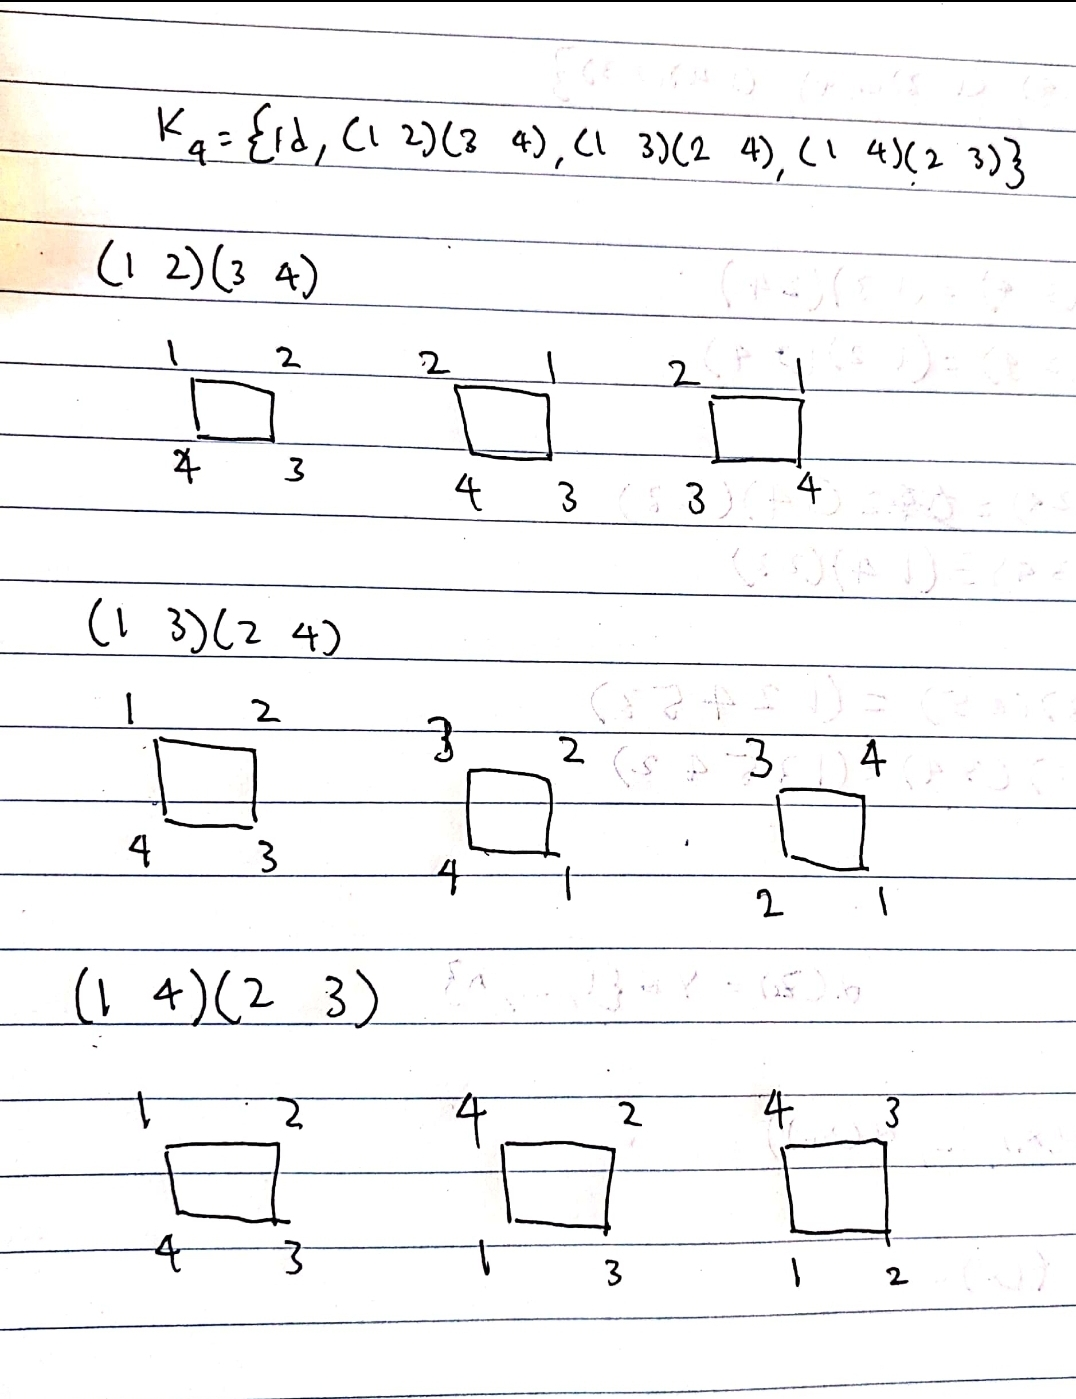
\includegraphics[scale=0.2]{img.jpg}
\end{figure}\\
For all 3 cases the vertices are still in the proper order. This way we can say that $K_4$ is a subgroup of $G$.
\newpage

\subsection*{Problem 7(A)}
I would probably start by having the students pair up a set of numbers or letters. Such as {1,2,3,4} or {a,b,c,d}. I would then ask the students to tell me how many pairings can they create. I would move on to slightly larger sets with 5 or 6 more elements and see how many can they come up with. I would then ask them how many pairings can you make if there are 50 or 100 things in a set. This would then prompt me to explain bout how the factorial function works. I would go on to explain that n! Is just the sum of products of all the numbers before it until 0. I would say that the reason the number of pairings you can make in a set is the factorial, is because, when you choose one number to pair with everything else, the next number has one less option. For example, if we try and pair the numbers {1,2,3,4} together, the number 1 has 4 possible numbers to get paired with, where as 2 only has 3. Hopefully they would understand this.

\subsection*{Problem 8(B)}
In highschool, the word permutation would normally align with “how many ways can I order something”, whether it be a line of books, or a stack of papers. In high school it would normally relate to a certain set of objects and how many different ways it can be ordered or put together, where each unique ordering is a permutation. Compared to group theory, highschool permutations are much simpler as they would normally focus on something finite or easy to picture. Whereas in group theory it is a much more abstract topic, permutations would normally refer to the composition of functions on a group, or the set of compositions between functions on a group. It would refer to the sequence of binary operations that exist within the group $S_n$. Although they both have different definitions and focus on very separate things. I would say that there is a small similarity between the two. Similar in the sense that both definitions look into how many different ways we can do “one” thing. For highschoolers it would be to order a set of objects, and for those who study group theory it would be looking at how many different ways and I impose the binary operation onto something.

\end{document}